\documentclass{article}
\usepackage[utf8]{inputenc}

\usepackage{graphicx}
\usepackage{float}
\usepackage{url}
\usepackage[margin=.75in]{geometry}
\usepackage{booktabs}

\usepackage{amsmath}
\usepackage{amssymb}
\usepackage{hyperref}
\usepackage{enumitem}
\usepackage{subcaption}
\usepackage{ulem}
\usepackage{xcolor}
\usepackage{soul}

\DeclareMathOperator*{\argmax}{arg\,max}
\DeclareMathOperator*{\argmin}{arg\,min}
\newcommand{\PP}{\mathbb{P}}
\newcommand{\prob}[1]{\PP \left( #1 \right)}
\newcommand{\condprob}[2]{\PP \left( #1 \middle| #2 \right)}
\newcommand{\EE}{\mathbb{E}}
\newcommand{\expect}[2]{\EE_{#1} \left[ #2 \right]}
\newcommand{\condexp}[3]{\EE_{#1} \left[ #2 \middle| #3 \right]}

\begin{document}
\begin{center}
	\begin{tabular}{|c|}
		\hline
		4180/5180: Reinforcement Learning and Sequential Decision Making (Fall 2024) \hspace{1cm} Christopher Amato \\
		Northeastern University \hfill  Due Oct 4, 2024                                                    \\\\
		{\bfseries \large Exercise 3: Dynamic Programming}                                    \\ \hline
	\end{tabular}
\end{center}

Please remember the following policies:
\begin{itemize}
	\item Exercise due at \textbf{11:59 PM EST Oct 4, 2024}.
	\item Submissions should be made electronically on Canvas. Please ensure that your solutions for both the written and programming parts are present. You can upload multiple files in a single submission, or you can zip them into a single file. You can make as many submissions as you wish, but only the latest one will be considered.
	\item For \uline{\textbf{Written}} questions, solutions should be typeset. 
	\item The PDF file should also include the figures from the \uline{\textbf{Plot}} questions.
	\item For both \uline{\textbf{Plot}} and \uline{\textbf{Code}} questions, submit your source code in Jupyter Notebook (.ipynb file) along with reasonable comments of your implementation. Please make sure the code runs correctly. 
	\item You are welcome to discuss these problems with other students in the class, but you must understand and write up the solution and code yourself. Also, you \textit{must} list the names of all those (if any) with whom you discussed your answers at the top of your PDF solutions page.
	\item Each exercise may be handed in up to two days late (24-hour period), penalized by 10\% per day late. Submissions later than two days will not be accepted.
	\item Contact the teaching staff if there are medical or other extenuating circumstances that we should be aware of.
	\item \textbf{Notations: RL2e is short for the reinforcement learning book 2nd edition. x.x means the Exercise x.x in the book.}
\end{itemize}

\begin{enumerate}
	\item \textbf{1 point.} (RL2e 3.25 -- 3.29) \textit{Fun with Bellman.} \\
	      \uline{\textbf{Written:}}
	      \begin{enumerate}
		      \item Give an equation for $v_*$ in terms of $q_*$.

		      \item Give an equation for $q_*$ in terms of $v_*$ and the four-argument $p$.

		      \item Give an equation for $\pi_*$ in terms of $q_*$.

		      \item Give an equation for $\pi_*$ in terms of $v_*$ and the four-argument $p$.

		      \item Rewrite the four Bellman equations for the four value functions ($v_\pi, v_*, q_\pi, q_*$) in terms of the three-argument function $p$ (Equation 3.4) and the two-argument function $r$ (Equation 3.5).

	      \end{enumerate}

	\item \textbf{1 point.} (RL2e 4.5, 4.10) \textit{Policy iteration for action values.} \\
	      \uline{\textbf{Written:}}
	      \begin{enumerate}
		      \item How would policy iteration be defined for action values? Give a complete algorithm for computing $q_*$, analogous to that on page $80$ for computing $v_*$. Please pay special attention to this exercise, because the ideas involved will be used throughout the rest of the book.

		      \item What is the analog of the value iteration update Equation 4.10 for action values, $q_{k+1}(s,a)$?

	      \end{enumerate}

	\item \textbf{2 points.} \textit{Policy iteration by hand.} \\
	      \uline{\textbf{Written:}}
	      Consider an undiscounted MDP having three states, $x, y, z$. %, with rewards $-1, -2, 0$, respectively.
	      State $z$ is a terminal state. In states $x$ and $y$ there are two possible actions: $b$ and $c$. The transition model is as follows:
	      \begin{itemize}
		      \item In state $x$, action $b$ moves the agent to state $y$ with probability $0.8$ \\
		            and makes the agent stay put (at state $x$) with probability $0.2$.
		      \item In state $y$, action $b$ moves the agent to state $x$ with probability $0.8$ \\
		            and makes the agent stay put (at state $y$) with probability $0.2$.
		      \item In either state $x$ or state $y$, action $c$ moves the agent to state $z$ with probability $0.1$ \\
		            and makes the agent stay put with probability $0.9$.
	      \end{itemize}
	      The reward model is as follows:
	      \begin{itemize}
		      \item In state $x$, the agent receives reward $-1$ regardless of what action is taken and what the next state is.
		      \item In state $y$, the agent receives reward $-2$ regardless of what action is taken and what the next state is.
	      \end{itemize}

	      Answer the following questions:
	      \begin{enumerate}
		      \item What can be determined \textit{qualitatively} about the optimal policy in states $x$ and $y$ (i.e., just by looking at the transition and reward structure, \textit{without} running value/policy iteration to solve the MDP)?

		      \item Apply policy iteration, showing each step in full, to determine the optimal policy and the values of states $x$ and $y$. Assume that the initial policy has action $c$ in both states.

		      \item What happens to policy iteration if the initial policy has action $b$ in both states? Does discounting help? Does the optimal policy depend on the discount factor (in this particular MDP)?

	      \end{enumerate}

	\item \textbf{2 points.} \textit{Implementing dynamic programming algorithms.} \\
	      \uline{\textbf{Code/plot:}}
	      For all algorithms, you may use any reasonable convergence threshold (e.g., $\theta = 10^{-3}$). We implement the $5 \times 5$ grid-world in Example 3.5 for you and please read the code in Jupyter Notebook for more details.
	      \begin{enumerate}
		      \item Implement \textit{value iteration} to output both the optimal state-value function and optimal policy for the given MDP (i.e., the $5 \times 5$ grid-world). Print out the optimal value function and policy for the $5 \times 5$ grid-world using your implementation ($v_*$ and $\pi_*$ are given in Figure 3.5). Please use the threshold value $\theta=1e^{-4}$ and $\gamma = 0.9$.
		      \item Implement \textit{policy iteration} to output both the optimal state-value function and optimal policy for the given MDP (i.e., the $5 \times 5$ grid-world). Print out the optimal value function and policy for the $5 \times 5$ grid-world using your implementation ($v_*$ and $\pi_*$ are given in Figure 3.5). Please use the threshold value $\theta=1e^{-4}$ and $\gamma = 0.9$.
	      \end{enumerate}

	\item \textbf{3 points.[5180]} (RL2e 4.7) \textit{Jack's car rental problem.}
	      \begin{enumerate}
		      \item \uline{\textbf{Code/plot:}} Replicate Example 4.2 and Figure 4.2. The implementation for Jack's car rental problem is given in the Jupyter Notebook. Please complete the policy iteration implementation to solve for the optimal policy and value function. Reproduce the plots shown in Figure 4.2 (The plotting functions are also given), showing the policy iterates and the final value function -- your plots do not have to be in exactly the same style, but should be similar (See the Figure below).
		      \item \uline{\textbf{Code:}} Re-solve Jack's car rental problem with the following changes. \\
		            \uline{\textbf{Written:}} Describe how you will change the reward function (i.e. compute\_reward\_modified function in the JackCarRental class) to reflect the following changes. \\
		            \uline{\textbf{Plot:}} Similar to part (a), produce plots of the policy iterates and the final value functions. \\
		            \uline{\textbf{Written:}} How does your final policy differ from Q5(a)? Explain why the differences make sense.
		            \begin{itemize}
			            \item One of Jack's employees at the first location rides a bus home each night and lives near the second location. She is happy to shuttle one car to the second location for free. Each additional car still costs $2$, as do all cars moved in the other direction.
			            \item In addition, Jack has limited parking space at each location. If more than $10$ cars are kept overnight at a location (after any moving of cars), then a total additional cost of $4$ must be incurred to use a second parking lot (independent of how many cars are kept there). (Each location has a separate overflow lot, so if both locations have $> 10$ cars, the total additional cost is $8$.)
		            \end{itemize}
		            These sorts of nonlinearities and arbitrary dynamics often occur in real problems and cannot easily be handled by optimization methods other than dynamic programming.
	      \end{enumerate}

	      \textit{Some clarification and guidance for completing Q5 and understanding the environment implementation}:
	      \begin{itemize}
		      \item The description of Jack's car rental problem in Example 4.2 is detailed, but some extra details are needed to reproduce the results shown in Figure 4.2. Assume the following daily schedule for the problem:
		            \begin{itemize}
			            \item 6 PM: ``End of day'': Close of business; this is when move actions are decided. \\
			                  From the description: ``The state is the number of cars at each location at the end of the day.''
			            \item 8 PM: Cars to be moved (if any) have arrived at their new location, including (in part b) by the employee going from location 1 to 2. \uline{The new location may have max $20 + 5$ cars after the move.}
			            \item 8 PM -- 8 AM: Overnight parking; in part b, need to pay $\$4$ for each location that has $> 10$ cars.
			            \item 8 AM: ``Start of day'': Open of business; one location may have up to $25$ cars.
			            \item 9 AM: All requests come in at this time (before any returns).
			            \item 5 PM: All cars are returned at this time, i.e., \uline{a returned car cannot be rented out on the same day}.
			            \item 5:59 PM: Excess cars ($> 20$) are removed at each location; each location has max $20$ cars.
		            \end{itemize}
		      \item Because of the somewhat larger state space and numerous request/return possibilities, a number of enhancements will likely be necessary to make dynamic programming efficient.
		            \begin{itemize}
			            \item The four-argument \textit{dynamics function} $p(s', r | s, a)$ is the most general form, but also the most inefficient form. In this case, using the three-argument \textit{transition function} $p(s' | s, a)$ (Equation 3.4) and the two-argument \textit{reward function} $r(s, a)$ will be \uline{much} more efficient. Use the Bellman equations for $v_\pi$ and $v_*$ in terms of $p(s' | s, a)$ and $r(s, a)$, derived in Q1(e), to replace the relevant lines in policy iteration.
			            \item The \textbf{compute\_expected\_return} function already computes the $p(s'|s,a)$ and $r(s, a)$ for your. Therefore, you only have to implement the incremental update of the expected return given $s$ and $a$.
			            \item In particular, the \textbf{open\_to\_close} function that computes, for a single location, the probability of ending the day with $s_\text{end} \in [0, 20]$ cars, given that the location started the day with $s_\text{start} \in [0, 20 + 5]$ cars. The function should also compute the average reward the location experiences during the day, given that the location started the day with $s_\text{start}$ cars. This ``open to close'' function can be pre-computed for all $26$ possible starting numbers of cars for each location. Then, to compute the joint dynamics between the two locations, all that is necessary is to consider the (deterministic) overnight dynamics, and then combine the appropriate ``open to close'' dynamics for each location. The function is implemented for you. But the description above will help you understand the implementation.
		            \end{itemize}
	      \end{itemize}

	      
	       \begin{figure}[h]
                 \centering
                 \begin{subfigure}[b]{0.4\textwidth}
                     \centering
                     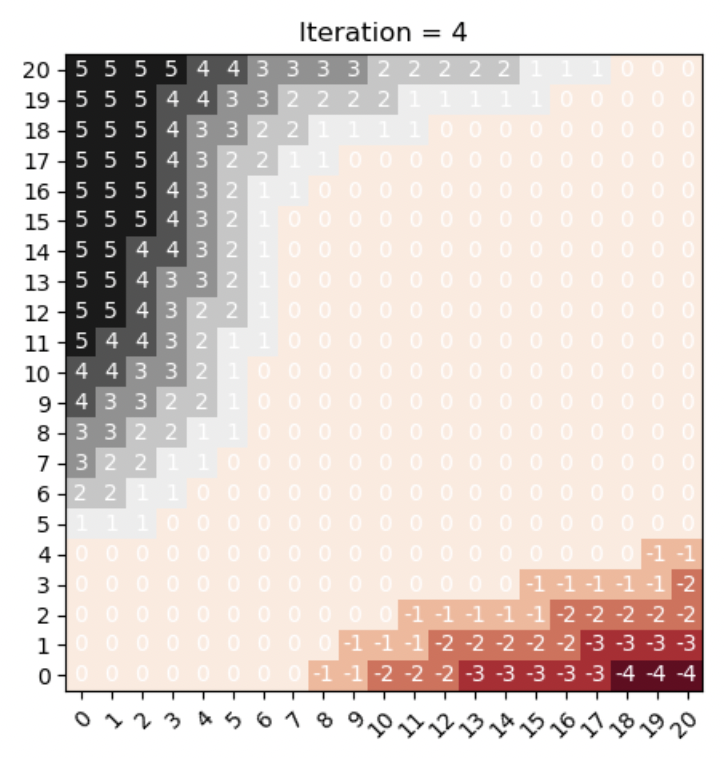
\includegraphics[width=\textwidth]{policy_vis.png}
                     \caption{Optimal policy}
                 \end{subfigure}
                 \begin{subfigure}[b]{0.4\textwidth}
                     \centering
                     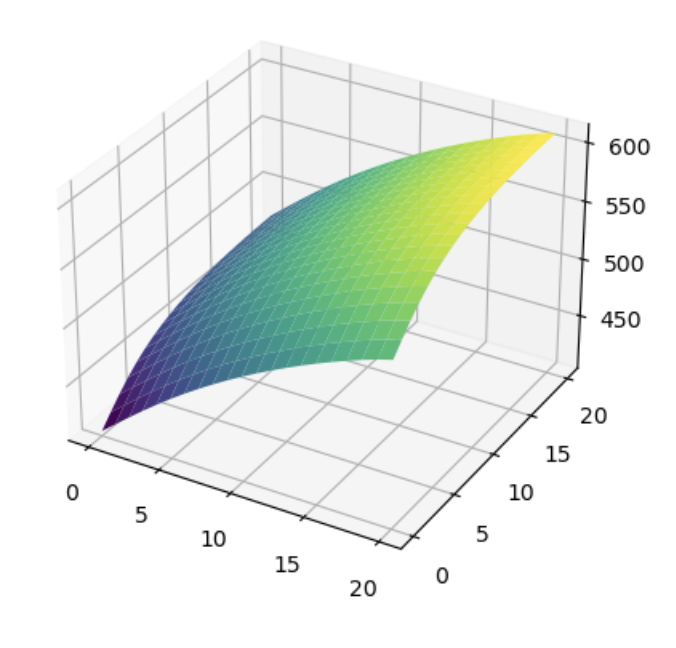
\includegraphics[width=\textwidth]{value_vis.png}
                     \caption{Optimal values}
                 \end{subfigure}
        \end{figure}

\item \textbf{1 point.} (RL2e 4.4) \textit{Fixing policy iteration.} \\
\uline{\textbf{Written:}}
\begin{enumerate}
\item The policy iteration algorithm on page 80 has a subtle bug in that it may never terminate if the policy continually switches between two or more policies that are equally good. This is okay for pedagogy, but not for actual use. Modify the pseudocode so that convergence is guaranteed.

\item Is there an analogous bug in value iteration? If so, provide a fix; otherwise, explain why such a bug does not exist.

\end{enumerate}

\item {{[Extra credit]} 2 points.} (AIMA 17.6) \textit{Proving convergence of value iteration.} \\
\uline{\textbf{Written:}}
\begin{enumerate}
\item Show that, for any functions $f$ and $g$,
\[ \left| \max_a f(a) - \max_a g(a) \right| \leq \max_a \left| f(a) - g(a) \right| \]
\textit{Hint}: Consider the cases $\max_a f(a) - \max_a g(a) \geq 0$ and $\max_a f(a) - \max_a g(a) < 0$ separately.

\item Let $V_k$ be the $k$'th iterate of value iteration (assume the two-array version for simplicity, i.e., there is no in-place updating).
Let $\mathcal{B}$ denote the \textit{Bellman backup operator}, i.e., the value iteration update can be written as (in vector form):
\[ V_{k+1} \leftarrow \mathcal{B} V_k \]
which is equivalent to applying the following assignment for all $s \in \mathcal{S}$:
\[ V_{k+1}(s) \leftarrow \max_a \sum_{s',r} p(s',r | s,a) \left[ r + \gamma V_k(s') \right] \]
Let $V_i$ and $V_i'$ be any two value function vectors. Using part (a), show that:
\[ \left\| \mathcal{B} V_i - \mathcal{B} V_i' \right\|_\infty \leq \gamma \left\| V_i - V_i' \right\|_\infty \]
(The $\ell_\infty$-norm of a vector $v$ is the maximum absolute value of its elements: $\| v \|_\infty \triangleq \max \{ |v_1|, |v_2|, \ldots, |v_n| \}$)

\item The result from part (b) shows that the Bellman backup operator is a \textit{contraction} by a factor of $\gamma$. \\
Prove that value iteration always converges to the optimal value function $v_*$, assuming that $\gamma < 1$. \\
To do this, first assume that the Bellman backup operator $\mathcal{B}$ has a fixed point $x$, i.e., $\mathcal{B} x = x$. \\
(The proof of this is beyond this scope of this course; see Banach fixed-point theorem for details.) \\
You should then show three things: value iteration converges to this assumed fixed point $x$, the fixed point is unique, and this unique fixed point is the optimal value function $v_*$.

\end{enumerate}
\end{enumerate}

\end{document}
